\section{State of the Art}
Grob betrachtet beinhalten verlustbehaftete Kompressionen drei Teilschritte: Transformation, Quantisierung und Entropie Kodierung. Die Abbildung \ref{state:aufbau} zeigt eine vereinfachte Abfolge. Die Inputdaten werden zuerst duch ein oder mehrere Verfahren transformiert. So transformieren, dass in der Quantisierung unwichtige Informationen entfernt werden können. Oft gehen nur im Quantisierungsschritt Daten verlohren, während alle anderen Schritte verlustfrei umkehrbar sind. Danach werden die Daten Entropie Kodiert. Für jeden Teilschritt gibt es unterschiedliche Verfahren. So können auch mehrere Transformationen hintereinander durchgeführt werden, oder eine ganze Folge von Transformations- und Quantisierungsverfahren.\\
\begin{figure}[!htbp]
	\center
	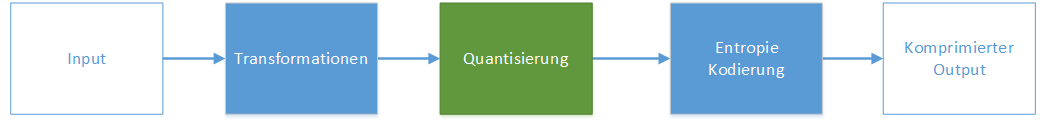
\includegraphics[width=0.8\textwidth,height=6cm,keepaspectratio]{./pictures/state/aufbau.png}
	\caption{Typische Teilschritte einer Kompression}
	\label{state:aufbau}
\end{figure}

\subsection{JPEG/JFIF Bildkompression}
\begin{figure}[!htbp]
	\center
	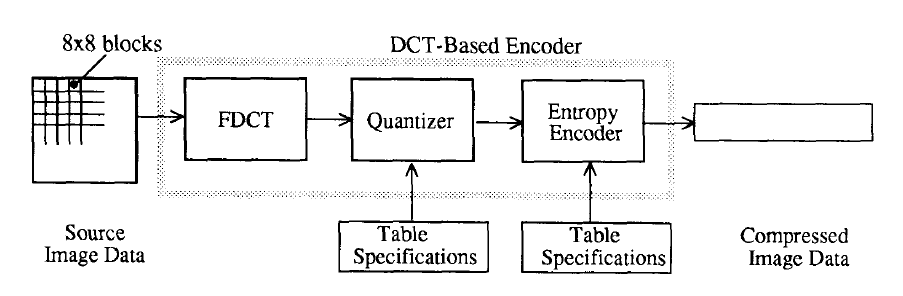
\includegraphics[width=0.8\textwidth,height=6cm,keepaspectratio]{./pictures/state/jpeg.png}
	\caption{Aufbau der JPEG Kompression \cite{wallace1992jpeg}}
	\label{state:jpeg:abb}
\end{figure}
Das JPEG/JFIF Bildformat ist eines der meist-verwendeten Bildkompressionsverfahren für natürliche Bilder. Das Diagramm der Abbildung \ref{state:jpeg:abb} zeigt den Aufbau der Kompressionspipeline. JPEG/JFIF unterteilt das Eingabebild in $8*8$ Blöcke und führt auf ihnen eine Diskrete Kosinus Transformation (DCT) durch. Der Bildblock ist nun als Folge von Kosinus-Funktionen dargestellt.\\
Die Quantisierung versucht nun Frequenzen, welche das menschliche Auge schlecht erkennen kann mit weniger Präzise darzustellen. Wenn die Quantisierung gut gewählt wurde, kann der Mensch das dekomprimierte Bild nicht vom Original unterscheiden, verbraucht aber weniger Speicherplatz. JPEG/JFIF bietet vorgefertigte Quantisierungstabellen an. Der Benutzer kann aber eigene Tabellen für spezifizieren. Wie die Quantisierungstabelle optimal gewählt wird, ist ein aktives Forschungsfeld \cite{wu1993rate:jpeg} \cite{wang2001designing:jpeg} und kann von Anwendungsfall zu Anwendungsfall unterschiedlich sein.\\
Nach der Quantisierung werden die quantisierten Blöcke im Zick-Zack-Muster angeordnet, sodass die Entropie Kodierung eine bessere Kompression durchführen kann. JPEG/JFIF führt eine Run-Length und eine Huffman-Kodierung durch. JPEG bietet auch hier an, eine benutzerspezifizierte Huffman-Tabelle zu verwenden.

wie das benutzt werden kann

\subsection{PointCloud Kompression}
Industrie Lasersampling
Bild pointcloud \cite{merry2006compression:pointcloud}
Grosse Punktmenge, welche im 3d Raum komprimiert werden soll.
verlustfrei/ Verlustbehaftet
Je nach Implementation können zu jedem Punkt zusatzinfos gespeichert werden wie Farbe/Normalen etc, darüber könnte die Information, zu welcher Linie ein Punkt gehört, gespeichert werden.

\subsection{Curve Fitting}
In der Signal Prozessierung Interpolation oder Rauschunterdrückung werden Signale mit Basisfunktionen.  \cite{unser1993b:spline} Schnelle B-Spline Signal interpolation und Approximation möglich. Wird aber in der Signal Processing weniger verwendet. Da kontinuierlich, können Operationen wie Integration und Diffenezierung direkt auf der Spline-Funktion durchgeführt werden. Noise reduktion möglich, aber auch Approximation. Verschiedene Ansätze die Knotenpunkte zu wählen (de boor)

\subsection{Signal Approximation}
Messtechnik von Medizin bis Fotografie, überall wo man ein Signal über Zeit hat
Versucht ein Signal durch eine Folge von Funktionen zu approximieren.

Gute Approximation kommt mit wenigen Funktionen aus.
Verlustbehaftete Kompression, indem man mit einer begrenzten Anzahl

fourier, wavelet Compressed sensing

\subsection{Entropie Kodierung}
Die Entropie Kodierung findet in allen Bereichen der Informatik Anwendungen. Allgemeien Verfahren RLE, Huffman, Arithmetic

Fix fertige Pakete wie Gzip, Rar welche meist mehrere Verfahren kombinieren.

Spezialisierte Entropie Kodierun:Fast Lossless floating point compression \cite{ratanaworabhan2006fast}